\documentclass[a4paper]{article}

%% Language and font encodings
\usepackage[english]{babel}
\usepackage[utf8x]{inputenc}
\usepackage[T1]{fontenc}

%% Sets page size and margins
\usepackage[a4paper,top=3cm,bottom=2cm,left=3cm,right=3cm,marginparwidth=1.75cm]{geometry}

%% Useful packages
\usepackage{amsmath}
\usepackage{graphicx}
\usepackage[colorinlistoftodos]{todonotes}
\usepackage[colorlinks=true, allcolors=blue]{hyperref}

%% other packaes
\usepackage{lineno}
\usepackage{float}
\usepackage{mathtools}
%\linenumbers

\title{Network Science applied to Biodivesity data}
\author{Pedro C. de Siracusa}

\begin{document}
\maketitle
\begin{abstract}
A modelagem de distribuição de espécies (SDM) nos permite identificar fatores ecológicos relevantes para o estabelecimento de espécies no meio ambiente, e a partir daí projetar mapas de provável distribuição atual ou futura. Estes modelos, construídos a partir de registros pontuais de ocorrências de espécies, são considerados ferramentas essenciais para a elaboração de políticas públicas para a conservação da biodiversidade, permitindo por exemplo avaliar o risco de extinção de espécies ou mesmo predizer respostas de comunidades biológicas a mudanças climáticas. Apesar da recente explosão no volume de dados de ocorrências de espécies, a baixa qualidade da maior parte destes registros impõe sérias restrições à sua utilização direta para a modelagem. O preprocessamento dos dados de ocorrências torna-se a etapa mais crítica no processo e envolve a validação de uma série registros individualmente, o que pode ser extremamente laborioso. Mecanismos de validação automatizada ou semi-automatizada poderiam ser elaborados utilizando regras de inferência sobre informações contextuais dos registros. Neste trabalho mostro como é possível compreender sistematicamente os contextos nos quais espécies são registradas a partir da estruturação de datasets de ocorrências de espécies como modelos de redes complexas. Utilizando como base o dataset do Herbário da Universidade de Brasília (UB) apresento a caracterização de redes de espécies e coletores sobre duas perspectivas. Na primeira perspectiva, redes espécie-coletor são representadas como grafos bipartite $B=(S_col, S_sp, E)$, em que $S_col$ é o conjunto de vértices que representam coletores; $S_sp$ é o conjunto de vértices que representam espécies; e $E$ o conjunto de arestas que ligam vértices de conjuntos diferentes.  Na segunda perspectiva, redes coletor-coautor são formadas a partir de registros co-autorados por coletores em campo. As redes estruturadas sobre ambas perspectivas apresentam características topológicas comuns a redes livres de escala, com poucos vértices muito conectados (hubs) e muitos vértices pouco conectados. Além disso, as perspectivas fornecem visões distintas. Redes espécie-coletor permitem identificar coletores que possuem interesse em espécies semelhantes, embora não necessariamente tenham coletado juntos. Inversamente, redes coletor-coautor permitem identificar coletores que de fato trabalham juntos em campo. 
\end{abstract}

\section{Introduction}

%% Current human activities in the environment are leading to the sixth mass extinction
%% Brazilian biodiversity is threatened by land loss, due to irresponsible agricultural practices, cattle farming, mineral extraction
%% Public policies towards conservation must prioritize areas and species for conservation
%%% Some species are still unknown by science or not sufficiently represented within protected areas
%%% Example: the biodiversity hotspots[Myers,200] and red lists




%% Data availability of species occurrence has substantially increased due to recent initiatives encouraging data curators to share species occurrence data(data sharing), citizen science...
%% Associated to the rise of the field of data science rises the tendency of the open model, which reinforces the need of collaboration in many sectors, including research. In research many initiatives for data sharing have been created \cite{Cao2017}, supporting an open science. 
%%% Massive quantities of biodiversity data is being made available
%%% Ecology is becoming a data-intensive science, requiring the use of data-driven approaches \cite{Kelling2009}	
%%% Data life cycle for transforming biodiversity data into knowledge \cite{Michener2012}

...
Recent advances in the fields of computer science and remote sensing technologies are significantly impacting the way in which scientific endeavor is pursued in many knowledge domains. 
The cheapening and shrinking of electronic components is currently pushing frontiers of how data is gathered in the domains of life and earth sciences, enabling researchers to have larger study areas covered with a multitude of higher-resolution autonomous networks of sensors \cite{Lehning2009}. 
These devices range from stationary weather stations, equipped with a set of environmental sensors for recording environmental data such as humidity and temperature, to camera traps for recording wildlife activity in photo and video formats.  
A significant increase in the rate at which environmental data is being produced stands out as a consequence of the rapid evolution of sensing devices towards their capacity of recording and storing larger volumes of data over longer time periods, without requiring human intervention. 
Such independence of human physical presence during the process of data collection also contributes for dropping data-associated costs, as field expeditions for maintenance purposes can be carried out less frequently, requiring shorter teams working for shorter periods.
...


% we're currently facing a shift in scientific culture to endorse open science and citizen science...
...
...


% Big data and e-science: many study domains face the data deluge... requiring new techniques for analysis
% Despite of the volume of available environmental and biotic data, a problematic is on what to do with such volume of data?
%% Public policies towards biodiversity conservation must be taken based on information (not data alone). 
%% We frequently lack a thorough scientific understanding of natural processes although we still need to take scientifically-informed decisions ('Science for Environmental Applications', 4th paradigm chapt.2)
%% Species occurrence data alone is not enough. The goal is to understand how environmental factors impact on organisms distribution
%% By understanding such factor we are able to prioritize more efficient policies and optimize cost-benefit
%%% For example must be able to predict species responses under the effect of environmental changes (e.g. global warming)
...
...

% SDM
%% Ecological Niche Modeling
%%% Models predict species occurrence based on environmental features
%%% We need to understand which are the most relevant factors driving species' distribution
%%% Species distribution in geographic space is inferred from relevant relationships discovered in environmental space
%%% Explain the term and equivalence to Species Distribution modeling
%%% Do SDMs model potential or realized niche?
%%% Why bother modeling instead of creating maps based on point interpolation?
...  ...   
 

Why use species distribution models?
  - Model the responses of species to environmental factors
  - Is an important tool for policy making towards biodiversity conservation
  - 
\todo{should I include some discussion on the main SDM algorithms?}

%% Some background on environmental data


%% Present the main algorithms for SDM 

\subsection{Current challenges on Species Distribution Modeling}

%There are two classes of limitations for working with museum data: errors and biases \cite{Newbold2010}.
%Currently available biodiversity occurrence data is rich for few localities (more sampling effort due to facilities), but extremely poor for many localities.
%Consequently knowledge about the occurrence of many species is limited to mostly sampled regions.
%This issue is known as the geographic sampling bias.
%There are some limitations for using museum data for species distribution modeling.
%Among the current challenges in species distribution modeling one concerns characterizing biases in biodiversity occurrence datasets.
%There are four most prevalent classes of bias sources. 
%Taxonomic or phylogenetic bias typically arises when collectors preferably record some group of species over others. 
...
Despite the high diversity of algorithms that have been adopted in literature for building species distribution models, drawing useful information from such models requires a thorough understanding not only on the assumptions and constraints inherent of the algorithms themselves, but also on the intrinsic limitations and peculiarities of the datasets used for fitting the models.
In experimental studies where a set of goals and hypotheses are stated in the initial phases of its elaboration, investigators often choose the most adequate sampling methods for investigating those particular scientific questions. %% random sampling designs... 

However, most of biodiversity occurrence data made freely available is provided by a growing number of initiatives sharing the mission of recording most of the species diversity as possible within the viability limits of their own resources. 
Instead of gathering data for investigating any previously defined scientific questions, they generate data for non-defined purposes, which in principle can be used by anyone for answering different kinds of questions.
Worldwide scientific collections and museums are taking efforts to digitize their collections and and making them available to remote users through data access platforms. % add examples
The growing number of citizen-science projects, besides enhancing the non-scientific community support towards science by engaging them in the data collection process, also provide an alternative for sampling broader regions while reducing associated sampling costs \cite{Silvertown2009a}. % add examples

%Such an opportunistic nature of museum data incurs in many caveats...
...




The main goals of this work [...]
% What are the main goals of this work?
%% Occurrence data context enrichment -> From network models, infer additional information about the context in which the record was obtained:
%%% Uncover collectors individual and collective trends from the data (Lambiotte2005)
%%%% Characterize the team of collectors responsible by the record? Are they specialists, students group...
%%%% From the profiles of the team of collectors and their recent activities could we infer something about the collection goals? Was it a big survey, a practical class...
%%%%%% e.g. A group of great specialists collecting together could characterize a big survey



This work provides an extension of the conceptual framework for networks sciences and coauthorship networks for studying networks of collectors in a biological collection dataset. And data enrichment. 
 

\section{Understanding Biodiversity Occurrence Data}

% Biodiversity occurrence data
%% Main data sources
%%% GBIF, Crowdsourcing (E-bird, Wikiaves, ...)

%%% Caveats: The importance of knowing the sampling methodology
%%%% Presence-only vs presence-absence records
%%%% Sources of bias in biodiversity occurrence data
%%%%%% Geographical bias, temporal bias, taxonomic bias, collector bias
    
% Define taxon, taxonomic rank, species, specimen...

%%% Availability of biodiversity data: data sources, data sharing, sensors...

Caveats on species distribution modeling
  - Many algorithms commonly used for SDM perform much better when both presence and absence data are provided. Due to the oportunistic nature of observational data we must provide pseudo-absence data. Pseudo-absence data is traditionally drawn from background. 

%% Caveat: The importance of knowing the sampling methodology
The importance of considering the sampling methodology used for gathering biodiversity data before providing it to any algorithm for SDM.
Depending on the sampling methodology used the set of records may assume distinct meanings.
The interpretation of the absence of a record is bound to the sampling methodology itself. 
Species presence is recordable, whereas absence is not.
Recording a particular species in a location is an unambiguous evidence of its existence, whereas not having recorded it in some other locations does not mean it does not occur there.

Species censuses usually generate higher-quality data in terms of species presence and absence, as collections are driven by probabilistic sampling designs designed for investigating some set of relevant questions. As an effect of their high cost, these are usually performed over lower-extent areas. 
As opposed to the experimental nature of how census data is traditionally gathered, most of biodiversity occurrence data publicly available have actually been collected opportunistically, without specific purposes or \textit{a priori}-stated hypotheses. 

Species census randomized sampling designs Such data is considered to be observational 
Observational data are far more volumous but are associated with a series of issues and biases.
Depending on the sampling design used for species recording, occurrence data is classified as either being presence-only or presence-absence. This is an important distinction.
The presence of a species in a location is a unambiguous evidence of its existence, whereas not having recorded it does not mean it does not occur there.

For many algorithms information on both the presence and absence of species are relevant.
However presence-only datasets are far more common, as they are usually derived from sets of opportunistic recordings. 


Regarding the availability of absence data, two distinct classes of input data that might be used to feed such models are presence-only data and presence-absence data.

Presence-only models must be especially accounted for bias as they are strongly influenced by it, whereas presence-absence are not so much. Therefore for presence-only models background data selection methods must ideally reflect the inherent bias of the occurrences dataset (instead of just using random background or pseudo-absences). Using target-groups background was shown to improve performance for some modeling methods \cite{Phillips2009}.
% check fig 4 in the paper %
 
\subsection{Data Quality}
 - Assessing data quality includes understanding user needs. \cite{KochVeiga2017}
 - Quality control across different features in an occurrences dataset is highly asymmetric. Greater effort is towards padronizing, validating and correcting features used for most applications (such as the species scientific name or latitude/longitude coordinates) if compared to normally unused fields, such as the names in the collectors field.
 
\section{Preparing data}
\subsection{Data Selection}
\subsection{Data Cleaning}


%% Names Atomizing
%%%% Extraction of names from names strings

%% User profiles matching (check paper "User profile matching in social networks) or Entity Resolution
%%% Retrieving names from the dataset: Problem statement
%%%% One complicating aspect is that entities identity information can only be derived from one feature (the recordedBy column). There are no unique identifiers associated to unique entities.
%%%% The recordedBy column only contains a string of collectors, in which names are not necessarily consistently separated. Names must be atomized...
%%%% Entity resolution
%%%% After atomization, another issue is that entities might exist in the dataset with different names:
%%%%%%% The identification problem \cite{Bhattacharya2007}: Finding all the possible name variations that are used to refer to an entity
%%%% Conversely, a single name might refer to multiple entities
%%%%%%% The disambiguation problem \cite{Bhattacharya2007}: Distinguishing multiple entities that are referred to by very similar (or even the same)  name
%%%%%%% The use of abbreviations in the recordedBy dataset potentializes this kind of problem.. e.g. 'J. Silva' might refer to João da Silva, José da Silva, Junior Silva, which are all very common brazilian names. 

%% Maybe a good idea to add figures to illustrate the problems!
...
In this section I describe my approach for cleaning data.
The models in this study are built using collectors names and species scientific names.

The quality of a field in biodiversity data depends on the data use.... \cite{KochVeiga2017}
Considerable work has been done on cleaning the species scientific name field, as it is widely used for species distribution modeling purposes.
On the other hand, fields holding collectors and identifiers ids are not usually important for most applications, and therefore not effort exists for improving the quality of this field.

The data cleaning process encompasses a set of routines for deriving entity names from columns in the dataset which store them as names strings.

...

\subsubsection{The Entity Resolution problem}
%% Entity resolution
%% Finding candidate heteronymous pairs
%%%% First an algorithm for name matching is executed. However, a good name matching alone is not enough for mapping two names to the same entity, and other attributes should also be included in a routine for detecting heteronymous entities \cite{Raad2010}.
%%%% Some last names are more common than others (such as Silva vs. Ratter)
%%%% SoftTFIDF metric worked well for multi-term names and the Jaro metric for single-term names in \cite{Raad2010}.
%%%% Attribute-based routines for profiles matching can be used in cases where we want to match user profiles over datasets by comparing their in terms of how similar their attributes sets are \cite{Bhattacharya2007}. 
%%%% A routine presented in \cite{Raad2010} allows specifying particular similarity metrics to attributes depending on their types and assigning them weights to account for their relevance in the matching process. Then aggregation functions can be used for deciding whether or not two profiles refer to the same entity.
%%%% However, in some cases we might want to use entities relational information for inferring their identities (based on the resolution of identities of the entities to which they correspond), what is known as collective entity resolution \cite{Bhattacharya2007}. This approach has been shown to outperform pure attribute-based approaches (cite same), especially for datasets with high ambiguity for the compared attributes. 
...
As defined by DarwinCore standards \cite{}, the names of collectors and identifiers responsible for, respectively, recording and identifying a specimen should be included as strings in fields named \textit{recordedBy} and \textit{identifiedBy}. According to the same standards, whenever multiple entities are to be included in a record for any of those fields their names must be included in a single string, separated with a consistent delimiter. DarwinCore standards recommend using the pipe character ("|") as delimiter, although in practice it is more relevant that the entire dataset uses a consistent delimiter for the entire records set. For example, if we wanted to include "Silva,T.J." and "Souza,L.M." as the collectors responsible for a record we could format the string as "Silva,T.J. ; Souza,L.M.", assuming the semicolon (";") character is also the delimiter for the rest of the records for this field. 

However, as collectors and identifiers names are traditionally not very relevant for most applications of biodiversity occurrence data, some data curators tend to overlook these fields, failing to invest enough effort for assuring their quality. As these fields do not contribute for significantly improving data fitness for most users, there is also a lack of data quality solutions addressing them \cite{KochVeiga2017}.
...
%% Names mapping
%%% By using a names map we define references from names variants to a normalized, adopted form.
%%% 

%% The names remapping is an iterative process, in which at each iteration a set of names identity is resolved
%% The similarity metric uses each node's neighborhood for inferring the probability that they refer to the same entity




\subsection{Features Selection}
In this step of the data preparation process my goal was to engineer features that could potentially be useful in subsequent steps. Next, from many features in the features space I need to select those which best represent the variety of collectors profiles.

\section{Network Models}
%% Collectors Profiling and activities history
%%%% Profiling collectors in terms of their activities and interests can be a way of further detecting anomalies (activity monitoring, Fawcett and Provost 1999).

This section contains the core models I've developed during this study.

Here a distinction must be stated for the terms "species" and "specimen" I'll constantly refer to along this text. The former refers to a taxonomic rank, a group of individuals forming a biological classification unit as determined by a professional taxonomist. The latter refers to an individual, which can be identified as being a representative of one species.

\subsection{The Science of Complex Networks: A theoretical background}
%% The rise of the field of complex networks
%% What are complex networks?
%%%% Random networks, small-world and scale-free topologies

% Networks are mathematically represented as graphs
%% Nodes and Edges
%%% Edges are established between a pair of nodes
%%% Nodes and edges can have attributes (each attribute holding values)
%%% Neighborhood, neighbors

%% Graph density
%%% Fully connected: n*(n-1)/2


%% Matrix Representation
%%% Adjacency matrix, sparsity

%% Degree
%%%% Degree distribution
%%%% Higher degree nodes (richer), lower degree nodes (poorer)

\subsubsection{Bipartite Graphs}
%% Bipartite graphs
%%%% The bipartite constraint: formalization: Nodes sets are DISJOINT (no intersection) ; and INDEPENDENT (no adjacent nodes within any set); 
%%%% Biadjacency matrix
%%%% Bipartite projection
%%%%%% bipartite projections edges set is usually very dense -> The importance of adding weights to edges in bipartite projections
%%%%%% weaker connections are then filtered out

  \begin{figure}[h!]
  	\centering
    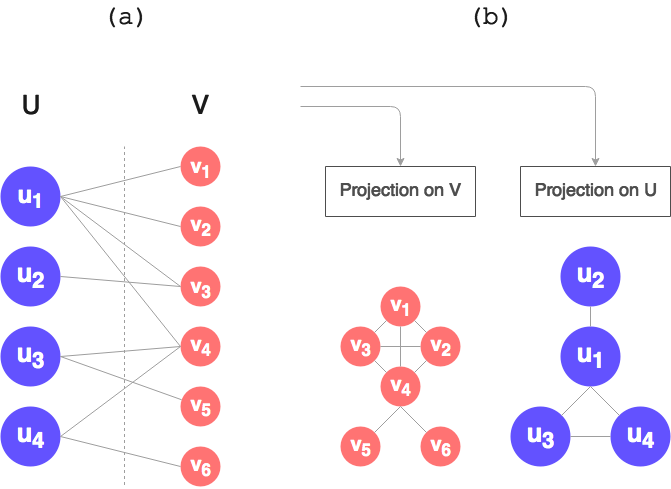
\includegraphics[width=0.5\linewidth]{figures/bipartite_general.png}
    \caption{(a) General aspect of a bipartite graph. All nodes in the graph belong to exactly one of $U$ and $V$ nodes sets. In addition edges are only established between nodes from distinct sets. (b) Bipartite projections. Projections onto each node set are constructed by linking together nodes that are at a length-2 distance in the bipartite graph, while omitting nodes from the other set.}
    \label{fig:bipartite_general}
  \end{figure}


\subsection{Species-collectors Networks}

%% Goals and Questions to investigate



\subsubsection{General description}

Species-collectors networks (SCN) describe relationships of the type "collector samples species" or, conversely, "species is sampled by collector". 
As such relationships can only possibly exist between collectors and species we explicitly represent collectors and species as entities belonging to distinct entity classes. Additionally, we add a constraint only allowing links to be established between collectors and species.
As all relationships in the network necessarily involve one entity belonging to each class it is best described by a bipartite graph model
$$ SCN = (S_{sp},S_{col},E)$$
where $S_{col}$ is the nodes set representing the collectors group; $S_{sp}$ is the nodes set representing the species group; and $E$ is the set of edges between members of $S_{col}$ and $S_{sp}$.

% https://www.latex-tutorial.com/tutorials/figures/
  \begin{figure}[h!]
  	\centering
    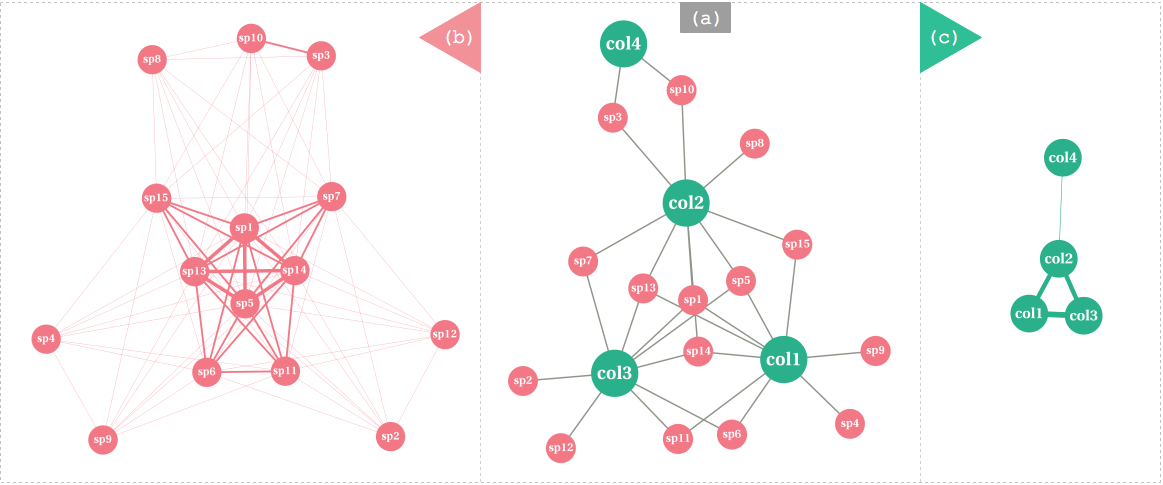
\includegraphics[width=\linewidth]{figures/scn_generalaspect.png}
    \caption{(a) General aspect of a species-collectors network model (SCN), where collectors are linked to the species they've recorded. The total number of records of a given species by some collector is reflected in the strength of their link. Here for simplicity all collectors have recorded each species once. (b) SCN projection onto the species set. Species are linked together if they've been collected by common collectors. Link strength is proportional to the number of collectors two species share. (c) SCN projection onto the collectors set. Collectors are linked together if they've recorded species in common. Link strength is proportional to the number of species two collectors share. Link strength in each network is graphically represented by edges thickness.}
    \label{fig:scn_general}
  \end{figure}

Note that in this model entities from the collectors class represent actual individuals (people), whereas each entity from the species class refer instead to a species, which by definition comprises a group of individuals. 
Therefore new links between nodes are formed whenever a collector records an individual belonging to a new species. 
For new occurrences of already existent species-collector pairs no new edges are added. Instead, the weights of those edges are increased, such that the final weight of each edge corresponds to the total number of times a given collector has recorded a given species.

Nodes and edges in a SCN model can also be represented as a \textit{biadjacency matrix} with dimensions $|S_{sp}|\times|S_{col}|$, with each element representing the number of records for a particular species by some collector.

Below I introduce some basic definitions in the scope of SCN models.

%% SCN definitions
\paragraph{Species bag.} 
The entire set and counts of species a collector has recorded in a dataset, which is equivalent to the set formed by the node's direct neighbors, composes his/her \textit{species bag}.
Species bag is an attribute which is exclusively derived for collectors nodes, formally defined as a vector
$$
\sigma^{(\mu)} =  \begin{bmatrix}
\sigma_1^{(\mu)}, \sigma_2^{(\mu)}, \cdots, \sigma_n^{(\mu)}
\end{bmatrix}  \quad : \quad 
n = |S_{sp}|
$$
where $n$ is the length of the species set and each $\sigma_i^{(\mu)}$ is the total number of records of species $i$ by collector $\mu$. 
The species bag can be directly obtained as a row-vector from the SCN biadjacency matrix.
The sum of all elements in a collector's species bag is given by the species bag's \textit{l1 norm} $|| \sigma^{(\mu)} ||_1$, and corresponds to the node's \textit{weighted degree} $k_w$.
 
\paragraph{Interest.} 
The entire set and counts of collectors that have recorded a particular species in a dataset is defined as its \textit{interest} vector. This concept can be thought as the inverse of a species bag, being equivalent to the nodes set formed by a species' direct neighbors. The interest vector is an attribute derived exclusively for species nodes, and is formally defined as
$$ 
\iota^{(\psi)} =  \begin{bmatrix}
\iota^{(\psi)}_1, \iota_2^{(\psi)}, \cdots, \iota_n^{(\psi)}
\end{bmatrix}  \quad : \quad 
n = |S_{col}|
$$
where $n$ is the length of the collectors set and each $\iota_i^{(\psi)}$ is the total number of records of species $\psi$ which was done by collector $i$. 
A particular species' interest can also be derived as a column-vector from the biadjacency matrix. 
The weighted degree $k_w$ of a species node can also be derived by computing the \textit{l1-norm} of its interest vector, such that $k_w^{(\psi)} \equiv || \iota^{(\psi)} ||_1 $.

\paragraph{Taxonomic aggregation and resolution.}
In some contexts it might be desired to simplify SCNs by grouping species nodes into higher taxonomic ranks (or levels), such as \textit{genus} or \textit{family}. This process is defined as \textit{taxonomic aggregation}, and is performed by 
($i$) obtaining a grouping of species using some taxonomic rank; 
($ii$) obtaining interest vectors for each species; 
($iii$) summing up interest vectors for all species in each group;
($iv$) building a new SCN model, aggregated on rank T. 
The SCN's \textit{taxonomic resolution} is the taxonomic rank at which species are aggregated in the model. For the sake of model interpretability, all species nodes must necessarily be represented as taxons belonging to the same rank as the SCN's taxonomic resolution.

For a more formal description let $G_T = \{ g_1, g_2, \cdots, g_n \}$ be a taxonomic grouping at rank $T$ containing a set of taxons $g_i$, each of them mapping to a set of species nodes $S_{sp}^{(i)} \subset S_{sp}$. Then for each node $g_i \in G_T$ we obtain their interest vectors by computing $ \iota^{(g_i)} := \sum_{j=1}^{m} \iota^{(v_j)} : v_j \in S_{sp}^{(i)}, m = |g_i|$. By stacking all interests vector as row-vectors we obtain a biadjacency matrix, which is then used to build a rank-T aggregated SCN model $SCN_T = (G_T,S_{col},E)$.
% The PICI model (Lambiotte2005)
%% Collective effects acting on individuals with similar interests
%% Individual mechanisms, pushing collectors towards their particular interests, establishing their collecting niche

% Temporal edges

% Bipartite projection
\subsubsection{Projections}

Although SCNs are originally built to model recording relationships between species and collectors, one might obtain additional insights by deriving indirect relationships from its structure. This is accomplished by projecting SCNs over each one of the nodes sets, as illustrated in Figure \ref{fig:scn_general} (b and c). Each projection gives us new perspectives on how strongly entities of the same type relate with each other in terms of their linkage patterns with intermediates.

A first perspective (Figure \ref{fig:scn_general} (b)) is obtained by projecting the graph onto the $S_{col}$ set, and allows us to investigate which collectors share interest in common sets of species. Collectors with at least one species in common in their species bags get directly connected, whereas species nodes are omitted. The second perspective (Figure \ref{fig:scn_general} (c)) represents species that are recorded by a common set of collectors or, in other words, share interest. Similarly to the other projection, projecting the SCN onto the $S_{sp}$ set directly links species with at least one collector in their interest vector while omitting collectors nodes.

In both projections link strength is given by some weighting rule, which can be applied depending on the question one wants to investigate. Below I first describe the simplest weighting rule with its limitations and, in sequence, some alternatives rules for overcoming them.
% https://doi.org/10.1016/j.physa.2006.12.021 <- The effect of weight on community structure of networks

\paragraph{Simple weighting.}
This rule assigns weights to links between pairs of collectors ($\mu_1$ and $\mu_2$) or species ($\psi_1$ and $\psi_2$) by simply counting the total number of species collectors share on their species bags or the total number of collectors species share in their interest vector. The rule is mathematically expressed as:
\begin{equation*}
\begin{split}
W_{(\mu_1, \mu_2)} &= \sum_{i=1}^{n} \delta(\sigma_i^{(\mu_1)}, \sigma_i^{(\mu_2)})\mbox{ , for the projection onto }S_{col}\mbox{ ;}\\
W_{(\psi_1, \psi_2)} &= \sum_{j=1}^{m} \delta(\iota_j^{(\psi_1)}, \iota_j^{(\psi_2)})
\mbox{ , for the projection onto }S_{sp}\mbox{, where}
\end{split}
\end{equation*}
$n = |S_{sp}|$, $m = |S_{col}|$ and 
$\delta(u,v) = 
\begin{cases}
1 & \mbox{if } u \times v > 0\\
0 & \mbox{otherwise}
\end{cases}
$ .

The simple weighting rule has two main limitations when applied to SCNs.
First, the weight assigned to edges linking pairs of nodes in the projection only reflects the number of different intermediate neighbors from the complementary set they shared in the non-projected graph. The number of times each species is recorded by each collector is ignored while computing the strength of links in the projections.
Second, such weighting rule tends to make very prolific and generalist collectors or very attractive species strongly connected to many others in a disproportional way, as an effect of their high degrees in the non-projected model. Besides overlooking the importance of more specialist nodes this rule also tends to make projected graphs very densely connected, which increases computational costs and obfuscates relevant relationships in the model. Analogous limitations were also reported for other bipartite social network models (\cite{Lambiotte2005}).
In order to reduce these effects we could instead use the alternative rules below.

\paragraph{Hyperbolic weighting.}
If a particular species is recorded by many different collectors or, conversely, if a particular collector has recorded many different species then we might want to

\paragraph{Species bag / Interest similarity.}
The \textit{species bag similarity} weighting rule reduces the effect of the degrees of a pair of nodes in their edge's weight by computing their similarity.
The metric of similarity between the species bags of two collectors $i$ and $j$ is defined as the \textit{cosine similarity}
$$
sim(\sigma^{(\mu_i)},\sigma^{(\mu_j)}) =
\cos \theta_{\mu_i,\mu_j} \equiv
\frac{  \sigma^{(\mu_i)} \cdot \sigma^{(\mu_j)}  }{  ||\sigma^{(\mu_i)}||_2  ||\sigma^{(\mu_j)}||_2  }
$$
where the outcome ranges from $[0,1]$. % Add mathematical description. If a weight was zero there would be no link. 
%%% check neighborhood similarity functions in literature

Projecting a SCN into the $S_{sp}$ set gives us a complementary perspective of relationships in the network.
Similarly to the $S_{col}$ projection, direct links between species are derived from their originally indirect, collector-mediated connections, where species having been recorded by at least one collector in common get linked together.
Edges are weighted according to similar rules as for the projection onto the $S_{col}$ set.
With this perspective we can investigate which species are most frequently associated to each other in species bags.% analogous to the shopping basket problem


Clustering algorithms can be used for identifying species that are usually collected by some group of collectors  




\subsection{Collectors Co-working Networks}
% References: (Ramasco2004)

%% Goals
%%% 1. I want to assign entities to profiles using attributes such as: Their betweeness, degree, tot_records. One problem is that entities forming communities in this model do not share such attributes: A community is formed by students, professors, great collectors...

%% Questions to investigate
%%% 1. Is there modularity for any attributes? (check Mislove, A.,et al 2010. You are who you know... sec 3) -> Instead of users modularity defined by them sharing attributes we could have them sharing species
%%% 2. Preferential attachment: Do new nodes tend to attach to higher-degree ones? This could be representing for example students beginning to collect with advisors/specialists.
%%% 3. Influence analysis: Who are the most influential nodes in the network? Do other entities tend to replicate the influencers' collecting behavior (at least on the beginning of their careers)? What is the global influence of the most influential collectors' bias in the herbarium?
%%% 4. Which features best reflect collectors expertise?

%% Temporal evolution
%%% Who the most influential collectors change with time?


In this section I describe Collectors co-working networks (CWN) as an approach for structuring networks of collectors co-authoring records in a species occurrence dataset. 
These models represent collectors as entities who correspond to each other by recording specimens in field collaboratively. 
In case a pair of collectors have co-authored any record in the dataset they are linked together with an undirected link.
For each pair of collectors there can be only one link, bearing a weight attribute which represents how many types that particular association is observed in the dataset.

Collaborative links are directly derived from fields describing the records collection authorship in occurrence datasets. 
According to \textit{DarwinCore} standards \cite{} this information should be stored as a string in a field named \textit{recordedBy}, where authors are separated from each other by a delimiter character.

These models have two main caveats. 
First, as opposed to species-collectors networks, collectors co-working networks model relationships between entities of the same type (collectors), and therefore information about the recorded specimens are not included in the links.
Second, collectors without at least one co-authorship association to any other collector are not represented in the model.

Collectors co-working network models are formally described as undirected graph objects
$$CWN = (S,E)$$
where $S$ and $E$ are the graph's nodes and edges sets representing, respectively, collectors and links between them. 

% Basic node attributes
The degree ($k$) for a node depends on the total number of edges it holds. 
This metric informs us how many different other collectors a collector has ever collaborated with.
In case we also want to consider the effect of the weights associated to each edge in the degree metric we must compute the weighted degree ($k_w$).
The \textbf{strength} of a node is the sum of the weights associated to all its edges. It describes the total number of collaborative records for a collector.
%% Average number of collaborators?





\subsection{Combining the network models}




\section{Case Study: The University of Brasília Herbarium (UB) dataset}
% herbarium page: http://florescer.unb.br/bol/

In this section I describe the application of the network models for deriving enriched information from the University of Brasilia Herbarium (UB) dataset.
The UB herbarium dataset is made publicly available for download through the Global Biodiversity Information Facility (GBIF) portal.
Here I assume the dataset has already been passed through a data cleaning process, and the entity resolution problem resolved.
Both CWN and SCN were built for supporting data enrichment.

Routines were written in Python3, using the Networkx and Pandas libraries.

According to the herbarium web page, the best represented families are:

\begin{itemize}
\item Araceae, collected and identified mainly by Gonçalves, E.G.;
\item Asteraceae;
\item Bignoniaceae;
\item Gramineae;
\item Lemnaceae, mostly collected and identified by Pott, V.J.;
\item Lythraceae, mostly collected and identified by Cavalcanti, T.B.;
\item Malpighiaceae, mostly collected and identified by Anderson, W.R.;
\item Melastomataceae;
\item Myrtaceae, mostly collected and identified by Proença, C.E.B. and Soares Silva, L.H.;
\item Orchidaceae, mostly collected and identified by Bianchetti, L.B., Menezes, L.C. and Batista, J.A.N.;
\item Leguminosae, mostly collected and identified by Irwin, H.S., Simon, M.F. and Valls, J.F.;
\item Rubiaceae, mostly collected and identified by Kirkbride Junior, J.H., Delprete, P., Souza, E.B., Cabral, E. and Salas, R.;
\item Viscaceae, mostly collected and identified by Caires, C.S.
\end{itemize}

\subsection{Dataset Characterization}

After loading the dataset with specified columns into memory I've filtered records with missing values for fields \textit{recordedBy} or \textit{scientificName}.
At the time of this study the resulting dataset had a total of 185301 records. However not all records have been identified up to the taxonomic resolution of \textit{species}, as shown in Table \ref{table:dset_taxonomicres_counts}. For the sake of interpretability of SCN models, we must only include entities that are representatives of the same taxonomic rank in the $S_{sp}$ nodes set, although it does not need to be necessarily the species rank. Therefore we must select records in the same taxonomic resolution of the SCN to build it.
Nodes can also be further grouped into higher-rank groups for model summarization, after the model is built. 

\begin{table}[H]
  \caption{Number of records for each taxonomic rank}
  \begin{center}
  \begin{tabular}{c c c}
       & count & \% \\
      \hline
      SPECIES & 140763 & 75.9645\\
      GENUS & 24397 & 13.1661 \\
      VARIETY & 8935 & 4.8219 \\
      FAMILY & 6223 & 3.3583 \\
      KINGDOM & 2008 & 1.0836 \\
      SUBSPECIES & 1681 & 0.9072 \\
      FORM & 1000 & 0.5397 \\
      PHYLUM & 294 & 0.1587 \\
      \hline
      total & 185301 & 100
  \end{tabular}
  \end{center}
  \label{table:dset_taxonomicres_counts}
\end{table}

For CWN models, on the other hand, the taxonomic resolution of each record is not relevant at all. All records can be used, irrespective of their taxonomic resolution.


%%% QUESTIONS

%% 1. How common are collaborative recordings within the dataset?
%%% What is the proportion of collaborative records in the dataset? How many collaborators
%%% One-collector recording vs >2 collectors recordings
%%% Distribution of team size
%%% Caveats: Some collectors may not include collaborators names in the records

%% 2.

%% x. Do collectors with similar interests tend to collect together?
%%% Mix of the two models
%%% Look for homophily in collectors communities, assortativity.

%% x. Which groups of species best modularize collectors in the dataset, in terms of their collection interests? 
%%% Using SCNs
%%% Are these groups necessarily taxonomic ones (such as family)? Or could functional groups be more relevant in some cases? Or is there a geographical effect?
%%% e.g. Some group might be best classified as specialists on species inhabiting some geographical location, with some specific habit and belonging to some family rather than simply as specialists in a given family.

%% x. The Expert-location problem {Chapt. 8 of book Social Network Data Analytics}
%%% The expert team formation problem: How can we best select experts for a given job, based on how willing they are of collaborating together?
%%% Combine both SCN and CWN


The Species-collectors network (SCN) 

% References {Newman2004}
% Statistical characterization of SCN structure
%% Species per collectors (species bag), collectors have species signatures
%% Collectors per species
%% Simply projecting this graph originates a very densely-connected network, failing to reveal relevant connectivity patterns (Lambiotte2005)

%% Define finer species taxonomic/functional division that best reflect collectors interests than division by family alone (Lambiotte2005)
%%% Do collectors interests communities reflect taxonomic divisions such as the family level?


% Statistical characterization of CWN structure
%% Largest component, connected components...
%% Assortativity: Do collectors with many collaborators (very collaborative) tend to associate with others that are also very collaborative?

% Network Evolution
%% Is network evolution ruled by preferential attachment?
%% How likely is it that two co-authors of a record will also be co-authors of another one?
%% Do attach influential collectors (high betweeness) attach preferentially to other influential ones? (Goh2003, Newman2004)


\subsection{Degree distribution?}

A first step for characterizing the network is to obtain its degree distribution.
The degree distribution was obtained for both 


\subsection{Who are the most central collectors in this herbarium?}





\subsection{Features Selection}

%% Features engineering







\section{Model Evaluation}

\section{Future perspectives}
% Building Recommending Systems
%% Collaborative filtering: The system gather information about the interest of the collectors and then proposes collectors to record new species based on the interests of others.



%%%%%%%%%% Glossary %%%%%%%%%%%%
%%%%%%%%%%%%%%%%%%%%%%%%%%%%%%%%

% Species bag: The entire set of species a collector has ever recorded

%%%%%%%%%%%%%%%%%%%%%%%%%%%%%%%%




%%%%%%%%%%  END %%%%%%%%%%%%%%%%
%%%%%%%%%%%%%%%%%%%%%%%%%%%%%%%%
%%%%%%%%%%%%%%%%%%%%%%%%%%%%%%%%
%%%%%%%%%%%%%%%%%%%%%%%%%%%%%%%%

\bibliographystyle{alpha}
\bibliography{lncc_thesis_bibliography}

\end{document}